% This is samplepaper.tex, a sample chapter demonstrating the
% LLNCS macro package for Springer Computer Science proceedings;
% Version 2.21 of 2022/01/12
%
\documentclass[runningheads]{llncs}
%
\usepackage[T1]{fontenc}
% T1 fonts will be used to generate the final print and online PDFs,
% so please use T1 fonts in your manuscript whenever possible.
% Other font encondings may result in incorrect characters.


% tightlist command for lists without linebreak
\providecommand{\tightlist}{%
  \setlength{\itemsep}{0pt}\setlength{\parskip}{0pt}}


% Pandoc citation processing
\newlength{\cslhangindent}
\setlength{\cslhangindent}{1.5em}
\newlength{\csllabelwidth}
\setlength{\csllabelwidth}{3em}
\newlength{\cslentryspacingunit} % times entry-spacing
\setlength{\cslentryspacingunit}{\parskip}
% for Pandoc 2.8 to 2.10.1
\newenvironment{cslreferences}%
  {}%
  {\par}
% For Pandoc 2.11+
\newenvironment{CSLReferences}[2] % #1 hanging-ident, #2 entry spacing
 {% don't indent paragraphs
  \setlength{\parindent}{0pt}
  % turn on hanging indent if param 1 is 1
  \ifodd #1
  \let\oldpar\par
  \def\par{\hangindent=\cslhangindent\oldpar}
  \fi
  % set entry spacing
  \setlength{\parskip}{#2\cslentryspacingunit}
 }%
 {}
\usepackage{calc}
\newcommand{\CSLBlock}[1]{#1\hfill\break}
\newcommand{\CSLLeftMargin}[1]{\parbox[t]{\csllabelwidth}{#1}}
\newcommand{\CSLRightInline}[1]{\parbox[t]{\linewidth - \csllabelwidth}{#1}\break}
\newcommand{\CSLIndent}[1]{\hspace{\cslhangindent}#1}

\usepackage{booktabs}
\usepackage{siunitx}
\usepackage{hyperref}
\hypersetup{colorlinks = TRUE,  urlcolor = blue, linkcolor = blue, citecolor = blue}

\usepackage{booktabs}
\usepackage{longtable}
\usepackage{array}
\usepackage{multirow}
\usepackage{wrapfig}
\usepackage{float}
\usepackage{colortbl}
\usepackage{pdflscape}
\usepackage{tabu}
\usepackage{threeparttable}
\usepackage{threeparttablex}
\usepackage[normalem]{ulem}
\usepackage{makecell}
\usepackage{xcolor}


\usepackage{graphicx}
% Used for displaying a sample figure. If possible, figure files should
% be included in EPS format.
%
% If you use the hyperref package, please uncomment the following two lines
% to display URLs in blue roman font according to Springer's eBook style:
\usepackage{hyperref}
\usepackage{color}
\renewcommand\UrlFont{\color{blue}\rmfamily}


\begin{document}


\title{biclaR: Estimating the socio-environmental impacts of car
substitution by bicycle and public transit using open tools}
%
\titlerunning{biclaR: SE impacts of car substitution by bicycle and
public transit}
% If the paper title is too long for the running head, you can set
% an abbreviated paper title here
%
\author{Rosa Félix\inst{1}\orcidID{0000-0002-5642-6006} \and Filipe
Moura\inst{1}\orcidID{0000-0001-7749-8490} \and Robin
Lovelace\inst{2}\orcidID{0000-0001-5679-6536}}


\authorrunning{R. Félix et al.}
% First names are abbreviated in the running head.
% If there are more than two authors, 'et al.' is used.
%

\institute{CERIS - Instituto Superior Técnico, University of Lisbon. Av
Rovisco Pais 1049-001 Lisboa, Portugal\\
\email{\href{mailto:rosamfelix@tecnico.ulisboa.pt}{\nolinkurl{rosamfelix@tecnico.ulisboa.pt}}}\\ \and Institute
for Transport Studies, University of Leeds. 34-40 University Rd, Leeds
LS2 9JT, UK}

\maketitle              % typeset the header of the contribution
%
\begin{abstract}
A high proportion of car trips can be replaced by a combination of
public transit and cycling for the first-and-last mile. This paper
estimates the potential for cycling combined with public transit (PT) as
a substitute for car trips in the Lisbon metropolitan area and assesses
its socio-environmental impacts using open data and open source tools. A
decision support tool that facilitates the design and development of a
metropolitan cycling network was developed (\emph{biclaR}). The social
and environmental impacts were assessed using the \emph{HEAT for
Cycling} and the \emph{HEAT as a Service} tools. The impacts of shifting
car trips to PT were also estimated and monetized. The results indicate
that 20\% of car trips could switch to the bicycle + PT combination.
Shifting to cycling for the first-and-last mile stages can reduce annual
CO\textsubscript{2}eq emissions from 6,000 tons/day, with benefits over
10 years of €230 million. For the PT leg, the transfer from car avoids
of at least 8,500 tons of CO\textsubscript{2}eq emissions per year. This
evidence can support policymakers to prioritize interventions that
reduce the reliance on private motor vehicles.

\keywords{Active transport \and Intermodality \and First and last
mile \and Health economic assessment \and Environmental
impacts \and Open data and methods}

\end{abstract}

\hypertarget{introduction}{%
\section{Introduction}\label{introduction}}

Combining public transportation (PT) and cycling for the first and last
mile in metropolitan areas can significantly replace private car trips.
This approach requires interventions and programs to make bicycling more
appealing, and the resulting public investments can have significant
social and environmental benefits.

According to the latest mobility survey conducted in 2018 {[}1{]}, the
LMA registered a total of 5.3 million daily trips, with only 0.5\% by
bicycle. Car modal share was 58.4\%, while PT accounted for 15.5\%. The
number of intra-municipal trips --- with origin and destination in the
same municipality --- amounts to 3.5 million trips. This exceeds the
number of inter-municipal trips (1.8 million trips), involving travel
between different municipalities. Cars and public transport are the most
used modes for intercity trips, with cars being the predominant choice
for all journeys.

To achieve the cycling targets set by the Portuguese national cycling
strategy for 2025 and 2030 (4\% and 10\%, respectively) {[}2{]}, the
Lisbon's Metropolitan Department of Transport introduced
\emph{biclaR}\footnote{See
  \href{https://biclar.tmlmobilidade.pt/}{biclar.tmlmobilidade.pt}.}, a
decision support tool that facilitates the design and development of a
metropolitan cycling network {[}3{]}.

\emph{biclaR} builds on the Propensity to Cycle Tool\footnote{See
  \href{https://www.pct.bike/}{pct.bike}.} (PCT), a web application and
research project funded by the UK's Department for Transport in 2015
which launched nationally in 2017 as part of the government's Cycling
and Walking Investment Strategy. The PCT initially used only
origin-destination data for commuting trips as the basis of estimates of
cycling potential at zone, route and route network levels {[}4{]}. The
PCT has been extended to include cycling potential for travel to school
in England {[}5{]} and other trip types in other countries.\footnote{See
  \href{https://www.npt.scot}{npt.scot} and
  \href{https://cruse.bike}{cruse.bike} for examples of the PCT in
  Scotland and Ireland that include estimates of cycling for other
  purposes.} However, to the best of our knowledge, this is the first
time that the method has been integrated with public transport data
using multi-modal routing to estimate the potential and benefits of
multi-stage cycling and PT trips.

This paper estimates the potential for combining cycling and PT to
substitute car trips in the LMA. After presenting the methods used, it
assesses its socio-environmental impacts using open data and open-source
tools.

\hypertarget{methods}{%
\section{Methods}\label{methods}}

\hypertarget{modeling-origin-destination-trips}{%
\subsection{Modeling Origin-Destination
trips}\label{modeling-origin-destination-trips}}

The mobility survey data {[}1{]} is the basis for this project and
defines the baseline scenario. Despite being conducted in the
pre-pandemic period (2017), this dataset represents the most
comprehensive and up-to-date information on urban mobility in Portuguese
metropolitan areas (Lisbon and Porto).

We used a method for disaggregating the origins and destinations of
trips between the centroids of two districts (same as ``parish'') to
ensure that a district is not solely characterized by a single point of
origin and destination for its trips. Aggregating all trips into
centroids renders the exercise less realistic, as it excludes a
significant portion of short-distance trips, a prevalent characteristic
of active mode travel {[}6{]}. The OD Jittering method breaks down a
single point (i.e., the centroid of an area) into multiple random points
on the existing and neighboring road network, using OpenStreetMap as a
reference. This method then distributes the volume of trips within the
district among the randomly generated origin-destination pairs.

Using the
\href{https://github.com/dabreegster/odjitter}{\texttt{odjitter} R
package}, we employed a maximum disaggregation level of 100 trips per
O-D pair for this project. Figure \ref{fig:jitter} illustrates the
contrast between trip representation through the traditional method,
which connects a single desire line between each district, and the
presentation achieved through the randomization and disaggregation of
trips between districts, specifically for the Lisbon metropolitan area.

\begin{figure}

{\centering 
\includegraphics[width=1\linewidth,]{img/jitter} 

}

\caption{Representation of OD pairs in the Lisbon metropolitan area between districts, without jittering (left) and with jittering (right).}\label{fig:jitter}
\end{figure}

Although this method provides a more realistic representation of the
trips undertaken compared to the traditional approach, it does not fully
align with the actual O-D pairs of trips, which remain unknown due to
data privacy regulations.

\hypertarget{modeling-routes}{%
\subsection{Modeling routes}\label{modeling-routes}}

The mobility survey collects the origin and destination of trips but
does not include the respective routes. Modeling the realistic cycling +
PT routes between OD pairs depends on assumptions regarding the
characteristics of the cycling and road networks and the location of
public transport interfaces. Other constraints regarding the behavior of
potential cyclists determine the routing results. For example, such
restrictions can favor low speed, low traffic streets, more direct
routes, and less steep paths, among others, suitable for cycling.

The selected route choice algorithm was the
\href{https://ipeagit.github.io/r5r/}{\texttt{r5r} R package} {[}7{]},
which allows for great flexibility in configuring estimated route types,
and which proven to provide most accurate route networks for the city of
Lisbon {[}8{]}. \texttt{r5r} can calculate multi-modal routes using PT
combined with other modes. It enables the identification of the most
direct or safest cycling routes, using the Level of Traffic
Stress\footnote{see
  \href{https://docs.conveyal.com/learn-more/traffic-stress}{docs.conveyal.com/learn-more/traffic-stress}.}
(LTS) scale, ranging from 1 to 4, where 1 corresponds to the quietest
(e.g., off-road cycle paths) and 4 corresponds to the least quiet (e.g.,
routes shared with motorized traffic). The routes were estimated for the
base scenario for both types of networks: \emph{direct} and \emph{safe},
using LTS 4 and LTS 3, respectively.

The \texttt{r5r} model used the OpenStreetMap road network and the GTFS
metropolitan data agregated and validated. This information is crucial
for an accurate PT trip and route estimation. A digital elevation model
from the European Space Agency's COPERNICUS mission, with a 25m spatial
resolution, was used to include street gradient information, as a weight
in cycling routing. The cycling potential trips for the two national
strategic targets (4\% and 10\%) was estimated from the values for
cycling and car trips (both as a driver and as a passenger) from the
2017 base scenario.

The routes were then overlaid and aggregated by segments, using
\href{https://docs.ropensci.org/stplanr/reference/overline.html}{\texttt{stplanr\ overline()}
R function}.

\hypertarget{modeling-intermodality}{%
\subsection{Modeling intermodality}\label{modeling-intermodality}}

The intermodality scenario considers trips combining PT and cycling for
the first and last legs. In a conservative approach, we have restricted
our analysis to the first and last legs with a combined length of up to
5 km (for instance: 1 km from origin to interface A plus 4 km from
interface B to destination) or up to 25 minutes on bike. Furthermore, we
have imposed restrictions on PT usage to include only trips with no PT
transfers, and up to 2 hours (120 min). Additionally, we have only
included PT modes that can easily accommodate bicycles, such as trains,
ferries, trams, and inter-municipal bus lines equipped with bike racks
(Figure \ref{fig:map1}).

\begin{figure}

{\centering 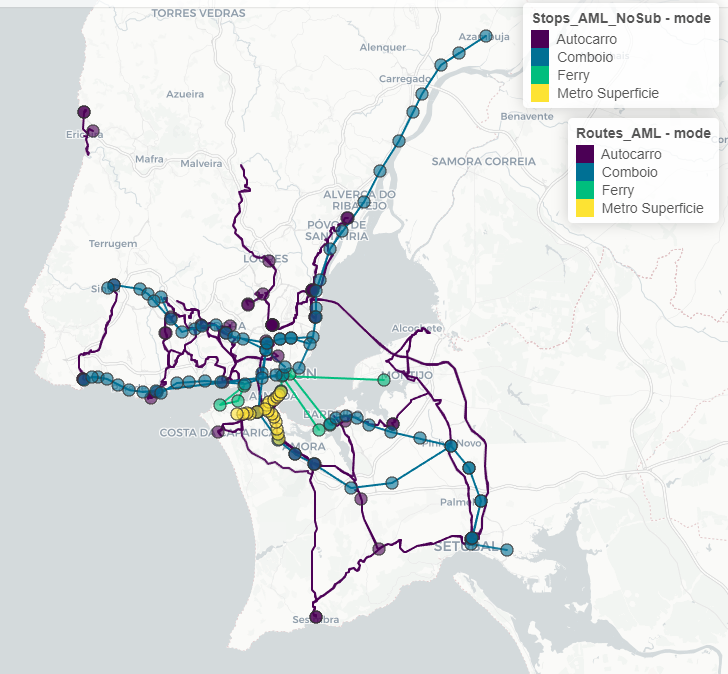
\includegraphics[width=0.6\linewidth,]{img/map1} 

}

\caption{Interfaces and lines considered, by transport mode, in the Lisbon metropolitan area}\label{fig:map1}
\end{figure}

Figure \ref{fig:map2} illustrates the resulting bicycle routes to access
the main PT interfaces in the LMA.

\begin{figure}

{\centering 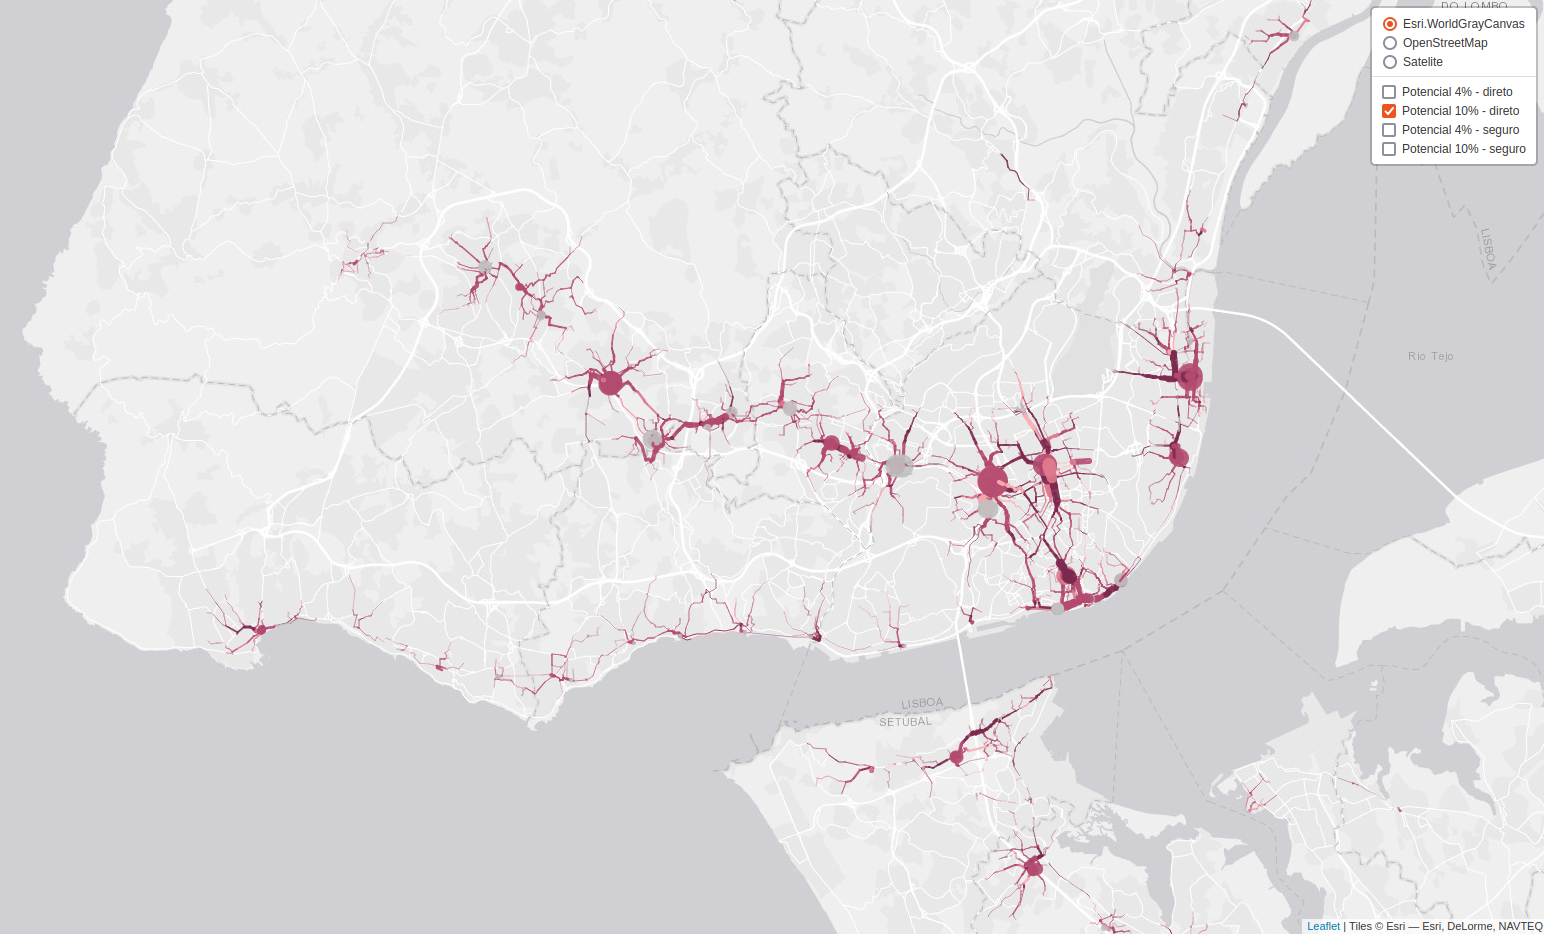
\includegraphics[width=0.8\linewidth,]{img/map2} 

}

\caption{Bike routes with highest potential to serve as first and last leg when replacing cycling and PT from car trips (screenshot of the interactive online tool).}\label{fig:map2}
\end{figure}

\hypertarget{assessing-socio-environmental-benefits}{%
\subsection{Assessing socio-environmental
benefits}\label{assessing-socio-environmental-benefits}}

For the cycling legs of the journey (first and last legs),
socio-environmental impacts were estimated, using the HEAT for Cycling
tool v5.0 {[}9{]} and the
\href{https://github.com/HEAT-WHO/HEAT_heatr_api}{\texttt{HEATaaS} R
package}\footnote{\texttt{HEATaaS} is under development. For more
  information contact
  \href{https://heatwalkingcycling.org}{heatwalkingcycling.org}.} from
the World Health Organization. The HEAT tool provided estimates on the
shifting from car to cycling for a short term time horizon (i.e., one
year) and the long term (i.e., ten years). We considered two dimensions:
\emph{social} --- including the physical activity of cyclists, air
pollution exposure, and road casualties; \emph{environmental} ---
including CO\textsubscript{2}eq emissions and other pollutants.

For the second leg of the journey, we estimate the additional
environmental impacts of shifting car trips to PT (between the PT
interfaces).

To estimate the car emissions, we used the EMEP/EEA's COPERT software v5
methods and reference values {[}10{]} for a Tier 3 detail level. We used
a family-size vehicle, EURO standard, and gasoline or diesel fuel. All
trips were considered to be made under urban conditions and at an
average speed of 15 km/h during rush hour periods. Since the average
distance traveled per trip influences the overconsumption and emissions
from cold-start engine operation, we estimated energy and emission
factors for different ranges of trips at 500-meter intervals. In
addition, we assumed an occupancy rate of 1.61 passengers \emph{per} car
{[}1{]}.

Regarding the PT, we considered the emission factor values reported in
the environmental and sustainability reports of the PT operators in the
LMA {[}11--14{]}.

Emissions were estimated for the following atmospheric pollutants:
CO\textsubscript{2}eq, CO, PM10, NOx, and VOC. In particular, for the
urban train and tram -- with 100\% electric traction -- only
CO\textsubscript{2}eq emissions were considered (resulting from the
production of electricity, considering a ``well-to-tank'' approach),
since the other pollutants are not emitted locally.

The conversion of avoided emissions into avoided welfare loss and
respective monetary valuation was based on the EU Guide to Cost-benefit
Analysis {[}15{]} and the best up-to-date reference values for the
various gases {[}15--17{]}. The social impacts are in avoided premature
mortality. This result is finally monetized using the \emph{Statistical
Value of Life} for Portugal {[}18{]}. We updated all the monetary
reference values of the literature based on the annual inflation rate in
Portugal for 2022\footnote{See
  \href{https://www.ine.pt/xportal/xmain?xpid=INE\&xpgid=ipc}{Statistics
  Portugal tool for inflation rate estimates between years}.}, and our
10-years estimations assumed a discount rate of 5\% and inflation of
3\%.

\hypertarget{results-and-discussion}{%
\section{Results and Discussion}\label{results-and-discussion}}

Table \ref{tab:summary1} presents the LMA total daily trips, the cycling
combined with PT trips in the baseline scenario and corresponding new
trips to achieve the national strategy targets (4\% and 10\%), for
different route profiles. For the cycling legs of the journey (first and
last legs), the environmental avoided emissions and monetized
socio-environment benefits are also presented, resulting from replacing
car trips with cycling.

\begin{table}

\caption{\label{tab:summary1}\label{summary1}Summary of the cycling potencial of intermodality scenario.}
\centering
\begin{tabular}[t]{llr>{\raggedleft\arraybackslash}p{6em}>{\raggedleft\arraybackslash}p{6em}>{\raggedleft\arraybackslash}p{6em}>{\raggedleft\arraybackslash}p{6em}}
\toprule
Target & Routing & Total trips & Baseline Cycling + PT & Potencial Cycling + PT & Avoided CO2eq (ton/yr) & SE Benefits for 10 years (thousand €)\\
\midrule
4\% & safe & 1 077 028 & 4 624 & 40 770 & 5 920 & 230 270\\
4\% & direct & 1 001 761 & 4 547 & 37 889 & 6 011 & 223 720\\
10\% & safe & 1 077 028 & 4 624 & 104 647 & 15 192 & 591 790\\
10\% & direct & 1 001 761 & 4 547 & 97 218 & 15 414 & 574 200\\
\bottomrule
\end{tabular}
\end{table}

For both \emph{direct} and \emph{safe} route profiles, 20\% of the daily
car trips have the potential to be replaced by a combination of PT and
cycling (up to 5 km on bike).

\emph{Table \ref{tab:summary21} shows something that doesn't make
sense.}

\begin{table}

\caption{\label{tab:summary21}\label{summary21}Summary of the potential of replacing car trips with cycling in combination with PT, disagregated by PT mode.}
\centering
\begin{tabular}[t]{ll>{\raggedleft\arraybackslash}p{4em}>{\raggedleft\arraybackslash}p{4em}>{\raggedleft\arraybackslash}p{4em}>{\raggedleft\arraybackslash}p{4em}>{\raggedleft\arraybackslash}p{4em}}
\toprule
Target & Routing & Total & Bus & Ferry & Train & Tram\\
\midrule
4\% & safe & 192 214 & 4 163 & 5 167 & 169 984 & 12 900\\
4\% & direct & 189 846 & 4 879 & 5 795 & 171 534 & 7 639\\
10\% & safe & 224 152 & 5 042 & 5 594 & 197 857 & 15 659\\
10\% & direct & 219 511 & 5 806 & 6 263 & 198 373 & 9 069\\
\bottomrule
\end{tabular}
\end{table}

This scenario unveils the potential of cycling as a complementary mode
of PT, with the potential to uptake the number of PT trips within the
LMA area by as much as 12\% (in addition to the 825 thousand PT trips
reported in the mobility survey). These findings indicate that
transferring car trips to a combination of bicycle and PT could be
nearly as substantial, if not equally significant, as the shift towards
bicycle-only trips.

When comparing the existing PT interfaces (Figure \ref{fig:map1}) with
the bike routes with highest potential to serve as first and last legs
(Figure \ref{fig:map2}) it becomes clear that the PT train interfaces
are the ones that have the highest potential to attract car-to-PT
substituting trips, if their accessibility by bicycle is improved to be
safe.

Table \ref{tab:summary22} presents the results of the avoided emissions
and its monetization for the second leg of the journey, by replacing car
trips with potential TP trips. Regarding the PT segment, the shift from
private car usage would lead to the mitigation of CO\textsubscript{2}
equivalent emissions to 8,500 to 20,800 tons annually, valued in €1.4
million to €3.5 million yearly, with trains offering the greatest
potential for substitution (88\%).

\begin{table}

\caption{\label{tab:summary22}\label{summary22}Summary of the avoided emmissions (ton/year) and corresponding monetization (thousand €) by replacing car trips with PT, in the second leg.}
\centering
\begin{tabular}[t]{ll>{\raggedleft\arraybackslash}p{3.5em}>{\raggedleft\arraybackslash}p{3.5em}>{\raggedleft\arraybackslash}p{3.5em}>{\raggedleft\arraybackslash}p{3.5em}>{\raggedleft\arraybackslash}p{3.5em}r}
\toprule
Target & Routing & CO2eq & CO & PM10 & NOx & VOC & Value (k€)\\
\midrule
4\% & safe & 8 593 & 17 & 1.9 & 27 & 0.8 & 1 425\\
4\% & direct & 8 702 & 18 & 2.0 & 28 & 0.8 & 1 453\\
10\% & safe & 20 627 & 42 & 4.6 & 65 & 2.0 & 3 431\\
10\% & direct & 20 793 & 42 & 4.7 & 66 & 1.9 & 3 487\\
\bottomrule
\end{tabular}
\end{table}

The sum of CO\textsubscript{2}eq avoided emissions from the potential
car trips shifted to bike (first-and-last legs) in combination with PT
(second leg) in the LMA is presented on Table \ref{tab:summaryall}, for
both national cycling strategy targets and routing profiles, and the
socio-environmental benefits monetized in €, for a 1-year and 10-year
time periods.

\begin{table}

\caption{\label{tab:summaryall}\label{summaryall}Summary of the avoided CO2eq emmissions (ton/year) and the estimated social and environmental benefits (monetized in thousand €) by replacing car trips with cycling in combination with PT.}
\centering
\begin{tabular}[t]{ll>{\raggedleft\arraybackslash}p{8em}>{\raggedleft\arraybackslash}p{8em}>{\raggedleft\arraybackslash}p{8em}}
\toprule
Target & Routing & Avoided CO2eq (tons) & SE Benefits 1yr (k€) & SE Benefits 10yrs (k€)\\
\midrule
4\% & safe & 14 513 & 27 299 & 242 024\\
4\% & direct & 14 713 & 26 572 & 235 706\\
10\% & safe & 35 819 & 69 938 & 620 094\\
10\% & direct & 36 207 & 67 956 & 602 972\\
\bottomrule
\end{tabular}
\end{table}

Shifting from car to cycling + PT can reduce annual
CO\textsubscript{2}eq emissions by 14,000 to 36,000 tons per year, and
the 10-year socio-environmental benefits account for €235 million to
€620 million, depending on the cycling targets.

\emph{Say something about the avoided C02eq emissions in the first and
last legs (bike) is about 3/4 of the PT leg avoided emissions, which is
(expected?) and should not be overlooked when promoting the use of PT.
Making the accessibility to PT interfaces more atractive to cycling and
providing bicycle-friendly equipments (parking) can reduce more 75\%
CO2eq emissions than the shifted car to PT trip} (FM/RL help)

Our findings suggest that a bicycle and PT combination could viably
replace 20\% of current LMA trips, with an additional 12\% of PT
journeys prone to further substitution.

\hypertarget{conclusion}{%
\section{Conclusion}\label{conclusion}}

The information on socio-economic benefits can support policy-makers in
prioritizing interventions to reduce the reliance on individual
motorized transportation, and better communicate their decisions by
providing the expected avoided GHG and air pollutant emissions and the
monetized socio-economic benefits for short and long terms. Different
routing profiles enable decision-makers to plan for different bicycle
user typologies and/or for different city cycling maturity levels
{[}19{]}.

The information available at \emph{biclaR} tool -- an open access
website -- can be downloaded and used with any GIS software to, for
instance, understand which potential cycling connections have the
highest socio-environmental impacts, in tons of avoided
CO\textsubscript{2}eq emissions, or in long term social benefits.

By making the research process publicly accessible in a code repository,
this research enables the replication of similar estimates for
socio-environmental impacts, resulting from a modal shift from car to
bicycle in combination with PT, in other metropolitan areas.

\hypertarget{acknowledgements}{%
\subsubsection*{Acknowledgements}\label{acknowledgements}}
\addcontentsline{toc}{subsubsection}{Acknowledgements}

This research was funded by the Lisbon's Metropolitan Department of
Transport (TML - Transportes Metropolitanos de Lisboa, E.M.T., S.A.),
under the \emph{biclaR} Project. This work is part of the research
activity carried out at Civil Engineering Research and Innovation for
Sustainability (CERIS) and has been funded by Fundação para a Ciência e
a Tecnologia (FCT), Portugal in the framework of project
UIDB/04625/2020. The authors thank Thomas Götschi (HEAT for Cycling) for
providing access to HaaS tool, which is under development.

\hypertarget{references}{%
\section*{References}\label{references}}
\addcontentsline{toc}{section}{References}

\hypertarget{refs}{}
\begin{CSLReferences}{0}{0}
\leavevmode\vadjust pre{\hypertarget{ref-IMOB}{}}%
\CSLLeftMargin{1. }%
\CSLRightInline{INE:
\href{https://www.ine.pt/xportal/xmain?xpid=INE\&xpgid=ine_publicacoes\&PUBLICACOESpub_boui=349495406\&PUBLICACOESmodo=2\&xlang=pt}{Mobilidade
e funcionalidade do território nas {Áreas Metropolitanas do Porto e de
Lisboa}: 2017}. {Instituto National de Estatística}, Lisboa (2018).}

\leavevmode\vadjust pre{\hypertarget{ref-ENMAC}{}}%
\CSLLeftMargin{2. }%
\CSLRightInline{Presidência do Conselho de Ministros: Resolução do
conselho de ministros n.º 131/2019,
\url{https://files.dre.pt/1s/2019/08/14700/0004600081.pdf}, (2019).}

\leavevmode\vadjust pre{\hypertarget{ref-felix2023}{}}%
\CSLLeftMargin{3. }%
\CSLRightInline{Félix, R., Lovelace, R., Moura, F.: {biclaR - Ferramenta
de apoio ao planeamento da rede ciclável na área metropolitana de
Lisboa}, \url{https://biclar.tmlmobilidade.pt}, (2022).}

\leavevmode\vadjust pre{\hypertarget{ref-lovelace2017}{}}%
\CSLLeftMargin{4. }%
\CSLRightInline{Lovelace, R., Goodman, A., Aldred, R., Berkoff, N.,
Abbas, A., Woodcock, J.: The Propensity to Cycle Tool: An open source
online system for sustainable transport planning. Journal of Transport
and Land Use. 10, (2017).
https://doi.org/\href{https://doi.org/10.5198/jtlu.2016.862}{10.5198/jtlu.2016.862}.}

\leavevmode\vadjust pre{\hypertarget{ref-goodman2019}{}}%
\CSLLeftMargin{5. }%
\CSLRightInline{Goodman, A., Rojas, I.F., Woodcock, J., Aldred, R.,
Berkoff, N., Morgan, M., Abbas, A., Lovelace, R.: Scenarios of cycling
to school in england, and associated health and carbon impacts:
Application of the {`}propensity to cycle tool{'}. Journal of Transport
\& Health. 12, 263--278 (2019).
https://doi.org/\href{https://doi.org/10.1016/j.jth.2019.01.008}{10.1016/j.jth.2019.01.008}.}

\leavevmode\vadjust pre{\hypertarget{ref-Lovelace2022Jittering}{}}%
\CSLLeftMargin{6. }%
\CSLRightInline{Lovelace, R., Félix, R., Carlino, D.: Jittering: A
computationally efficient method for generating realistic route networks
from origin-destination data. Findings. (2022).
https://doi.org/\href{https://doi.org/10.32866/001c.33873}{10.32866/001c.33873}.}

\leavevmode\vadjust pre{\hypertarget{ref-r5r}{}}%
\CSLLeftMargin{7. }%
\CSLRightInline{Pereira, R.H.M., Saraiva, M., Herszenhut, D., Braga,
C.K.V., Conway, M.W.: r5r: Rapid realistic routing on multimodal
transport networks with R5 in r. Findings. (2021).
https://doi.org/\href{https://doi.org/10.32866/001c.21262}{10.32866/001c.21262}.}

\leavevmode\vadjust pre{\hypertarget{ref-Lovelace2022exploring}{}}%
\CSLLeftMargin{8. }%
\CSLRightInline{Lovelace, R., Félix, R., Carlino, D.: Exploring
jittering and routing options for converting origin-destination data
into route networks: Towards accurate estimates of movement at the
street level. The International Archives of the Photogrammetry, Remote
Sensing and Spatial Information Sciences. XLVIII-4/W1-2022, 279--286
(2022).
https://doi.org/\href{https://doi.org/10.5194/isprs-archives-XLVIII-4-W1-2022-279-2022}{10.5194/isprs-archives-XLVIII-4-W1-2022-279-2022}.}

\leavevmode\vadjust pre{\hypertarget{ref-HEAT}{}}%
\CSLLeftMargin{9. }%
\CSLRightInline{Kahlmeier, S., Götschi, T., Cavill, N., Castro
Fernandez, A., Brand, C., Rojas Rueda, D., Woodcock, J., Kelly, P.,
Lieb, C., Oja, P., others:
\href{https://www.euro.who.int/__data/assets/pdf_file/0010/352963/Heat.pdf}{Health
economic assessment tool ({HEAT}) for walking and for cycling: Methods
and user guide on physical activity, air pollution, injuries and carbon
impact assessments}. (2017).}

\leavevmode\vadjust pre{\hypertarget{ref-COPERT}{}}%
\CSLLeftMargin{10. }%
\CSLRightInline{Ntziachristos, L., Samaras, Z.: {EMEP/EEA} air pollutant
emission inventory guidebook 2019,
\url{https://www.emisia.com/utilities/copert/documentation/}, (2020).}

\leavevmode\vadjust pre{\hypertarget{ref-Carris2019s}{}}%
\CSLLeftMargin{11. }%
\CSLRightInline{Carris:
\href{https://www.carris.pt/media/dkdp2wbg/dnf_carris2019_rv5.pdf}{Relatório
de sustentabilidade 2019 - demostração não financeira}. {Carris -
Companhia Carris de Ferro de Lisboa, E.M., S.A.} (2020).}

\leavevmode\vadjust pre{\hypertarget{ref-Metro2019s}{}}%
\CSLLeftMargin{12. }%
\CSLRightInline{Metropolitano de Lisboa:
\href{https://www.metrolisboa.pt/wp-content/uploads/2021/01/relatorio_integrado_2019.pdf}{Relatório
integrado 2019}. {Metropolitano de Lisboa, E.P.E.} (2020).}

\leavevmode\vadjust pre{\hypertarget{ref-CP2019s}{}}%
\CSLLeftMargin{13. }%
\CSLRightInline{CP:
\href{https://www.cp.pt/StaticFiles/Institucional/2_gestao_sustentavel/1_RelatoriosSustentabilidade/relatorio-de-sustentabilidade-2019.pdf}{Relatório
de sustentabilidade 2019}. {CP - Comboios de Portugal, E.P.E.} (2020).}

\leavevmode\vadjust pre{\hypertarget{ref-Transtejo2014}{}}%
\CSLLeftMargin{14. }%
\CSLRightInline{Transtejo:
\href{https://ttsl.pt/wp-content/uploads/2018/01/rs_2014_min.pdf}{Relatório
de sustentabilidade 2014}. {Grupo Transtejo, S.A.} (2014).}

\leavevmode\vadjust pre{\hypertarget{ref-EuropeanCommission2014}{}}%
\CSLLeftMargin{15. }%
\CSLRightInline{Sartori, D., Catalano, G., Genco, M., Pancotti, C.,
Sirtori, E., Vignetti, S., Del Bo, C.:
\href{https://ec.europa.eu/regional_policy/sources/docgener/studies/pdf/cba_guide.pdf}{Guide
to cost-benefit analysis of investment projects. Economic apraisal tool
for cohesion policy 2014-2020}. {European Commission - Directorate
General for Regional and Urban Policy} (2014).}

\leavevmode\vadjust pre{\hypertarget{ref-bickel2006}{}}%
\CSLLeftMargin{16. }%
\CSLRightInline{Bickel, P., Friedrich, R., Burgess, A., Fagiani, P.,
Hunt, A., Jong, G.D., Laird, J.:
\href{https://trimis.ec.europa.eu/sites/default/files/project/documents/20130122_113653_88902_HEATCO_D5_summary.pdf}{{HEATCO
- Developing Harmonised European Approaches for Transport Costing and
Project Assessment. Deliverable 5, Proposal for Harmonised Guidelines.}}
(2006).}

\leavevmode\vadjust pre{\hypertarget{ref-UNITE}{}}%
\CSLLeftMargin{17. }%
\CSLRightInline{Nash, C., others:
\href{https://www.its.leeds.ac.uk/projects/unite/downloads/Unite\%20Final\%20Report.pdf}{UNIfication
of accounts and marginal costs for transport efficiency: Final report}.
{Institute for Transport Studies, University of Leeds} (2003).}

\leavevmode\vadjust pre{\hypertarget{ref-ANSR2021}{}}%
\CSLLeftMargin{18. }%
\CSLRightInline{Silva, C., Bravo, J.V., Gonçalves, J.:
\href{http://www.ansr.pt/Estatisticas/RelatoriosTematicos/Documents/O\%20Impacto\%20Economico\%20e\%20Social\%20da\%20Sinistralidade\%20-\%20PT.pdf}{{Impacto
Económico e Social da Sinistralidade Rodoviária em Portugal}}. {CEGE -
Centro de Estudos de Gestão do ISEG, Autoridade Nacional de Segurança
Rodoviária (ANSR)} (2021).}

\leavevmode\vadjust pre{\hypertarget{ref-felix2017}{}}%
\CSLLeftMargin{19. }%
\CSLRightInline{Félix, R., Moura, F., Clifton, K.J.: Typologies of urban
cyclists: Review of market segmentation methods for planning practice.
Transportation Research Record. 2662, 125--133 (2017).
https://doi.org/\href{https://doi.org/10.3141/2662-14}{10.3141/2662-14}.}

\end{CSLReferences}

%
% ---- Bibliography ----



\end{document}
